% This line sets the project root file.
% !TEX root = Notes_Gauging_Defects.tex
% !TEX spellcheck = en_US

\subsection{Bimodule tensor products}\label{sec:bimodtensor}

To extend a category $\cat$ to include bimodule objects, we need to introduce `bimodule trivalent vertices'. To construct these, we need a product on bimodules. 

\begin{definition}[Relative tensor product]
	Given bimodules $\mathcal{A}\curvearrowright\mathcal{M}\curvearrowleft\mathcal{B}\curvearrowright{\mathcal{N}}\curvearrowleft\mathcal{C}$, the \emph{relative tensor product} $\mathcal{M}\otimes_\mathcal{B}\mathcal{N}$ has objects $(m,n)\in \mathcal{M}\otimes\mathcal{N}$, along with isomorphisms $\beta:(m\triangleleft b,n)\cong(m,b\triangleright n)$. The isomorphisms should be compatible with the module structure, for example
	\begin{align}
	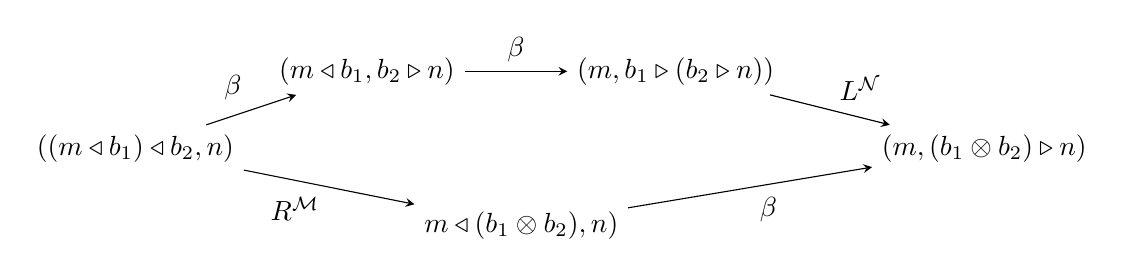
\begin{tikzpicture}[scale=.98,baseline=(current bounding box.center)]
	\node (A) at (-1,0) {$((m\triangleleft b_1)\triangleleft b_2,n)$};
	\node (B) at (2,1) {$(m\triangleleft b_1,b_2\triangleright n)$};
	\node (C) at (6,1) {$(m,b_1\triangleright(b_2\triangleright n))$};
	\node (D) at (10,0) {$(m,(b_1\otimes b_2)\triangleright n)$};
	\node (E) at (4,-1) {$m\triangleleft (b_1\otimes b_2), n)$};
	\draw [-stealth,above left] (A)--(B) node [pos=.5] {$\beta$};
	\draw [-stealth,above] (B)--(C) node [pos=.5] {$\beta$};
	\draw [-stealth,above right] (C)--(D) node [pos=.5] {$L^\mathcal{N}$};
	\draw [-stealth,below left] (A)--(E) node [pos=.5] {$R^{\mathcal{M}}$};
	\draw [-stealth,below right] (E)--(D) node [pos=.5] {$\beta$};
	\end{tikzpicture},
	\end{align}
	commutes. Here, $L^\mathcal{N}$ denotes the associator for the left action in $\mathcal{N}$ and $R^\mathcal{M}$ denotes the associator for the right action in $\mathcal{M}$. Morphisms in $\mathcal{M}\otimes_\mathcal{B}\mathcal{N}$ are morphisms in $\mathcal{M}\otimes\mathcal{N}$ that are compatible with $\beta$. $\mathcal{M}\otimes_\mathcal{B}\mathcal{N}$ is an $\mathcal{A}$-$\mathcal{C}$ bimodule, and can be decomposed into simple bimodules $\mathcal{P}$  $$\mathcal{M}\otimes_\mathcal{B}\mathcal{N}\cong\oplus_\mathcal{P}N_{\mathcal{M},\mathcal{N}}^\mathcal{P}\mathcal{P},$$
	where the $N_{\mathcal{M,N}}^\mathcal{P}$ are the corresponding coefficients in the decomposition. A complete definition can be found in \cite{DSPS14}.
\end{definition}

If a given bimodule $\mathcal{P}$ occurs in the decomposition of $\mathcal{M}\otimes_\mathcal{B}\mathcal{N}$, it is natural to introduce bimodule trivalent vertices of the form
\begin{align}
\begin{tikzpicture}[baseline=(current bounding box.center)]
\node (A) at (-.707,-.707) {$m\in\mathcal{M}$};
\node (B) at (.707,-.707) {$n\in\mathcal{N}$};
\node (C) at (0,1) {$p\in\mathcal{P}$};
\draw[violet,line width=0.4mm](A)--(0,0);
\draw[brown,line width=0.4mm](B)--(0,0);
\draw[nicegreen,line width=0.4mm](0,0)--(C);
\end{tikzpicture}.
\end{align}
This is the essence of the `inflation trick' developed in \cite{BBJ18,BB19a,BB19b}. We refer the interested reader to these references for more details. 